\section{Kép összehasonlítás}

Az alkalmazásnak képesnek kell lennie egyszerű kép összehasonlításra, hogy a felhasználó kapjon valamilyen visszajelzést arról, hogy elékszült-e a feladattal. Természetesen száz százalék pontosságot nem lehet elvárni se a felhasználától, se az algoritmusoktól, így a hibahatárt harminc százalékra állítottam. Hetven százalékos egyezés esetén a megoldást már elfogadottnak tekintjük. Fontos kikötés, hogy az összehasonlítás során mindkettő képnek azonos felbontásúnak kell lennie, különben a képet át kellene méretezni, ami artifactek-kel járhat. Ez megint csak megnehezítené a kép összehasonlítás már alapból nehéz feladatát.

\subsection{Chi square distance}

A chi square distance algoritmust a \ref{eq:chi square distance} képlet szemlélteti.

\begin{equation} \label{eq:chi square distance}
    CSD(x,y) = \sum_{i=1}^{n} = \frac{(x_i - y_i)^2}{y_i}\cite{CSQD}
\end{equation}

ami egy RGBA komponensű képre a \ref{eq:rgbacsd} képlet.

\begin{equation} \label{eq:rgbacsd}
\begin{gathered}
RGBACSD(x,y) = \\
CSD(x_r, y_r) + CSD(x_g, y_g) + CSD(x_b, y_b) + CSD(x_a, y_a)
\end{gathered}
\end{equation}


Sajnos az algoritmus olyan rosszul teljesít, amennyire egyszerű. Forgatásra, eltolásra, tükrözésre nem érzékeny és kicsi változtatásokra is nagy eltérést tud mutatni.

Az algoritmust egy \mintinline{cpp}{ImageComparator} osztályban implementáltam. Az implementáció első része, hogy a kép minden színcsatornájából egy hisztogrammot készítek, melyet egy struktúrával valósítottam meg. Esetemben minden kép RGBA komponensekből áll, tehát minden pixel négy bájt és minden bájt az RGBA komponens egyik színértékét ábrázolja mint ahogy ez látható a \ref{fig:rgba} ábrán. Így csak létrehozok minden színcsatornának egy \(2^8 - 1 = 255\) elemű tömböt aminek minden eleme nullára van inicializálva és a színértéknek megfelelő tömb indexen lévő értéket inkrementálom eggyel. Minden csatorna esetén csak a kinyerni kívánt csatorna első értékének a helyétől kell a ciklust indítani és minden iterációban a ciklus változót a komponens hosszával növelni.


\begin{figure}[hbt!]
    \centering
    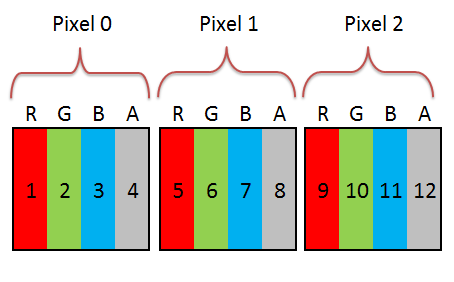
\includegraphics[width=0.75\textwidth,height=0.75\textheight,keepaspectratio]
    {resources/color_channels.png}
    \caption{RGBA komponens felépítése\cite{RGB}}
    \label{fig:rgba}
\end{figure}

Miután megvannak a hisztogramm struktúráink, csak a fentebbi képlet alapján kiszámolunk egy értéket minden csatornára, majd összegezzük az összes színcsatornára kapott eredményt és visszatérünk vele. 

A kapott érték egy \([0,width * height * maxColorValue * componentLength]\) intervallum közötti lebegőpontos érték. Két kép akkor számít azonosnak ha a kapott érték nyolc tized vagy annál kissebb.

\subsection{Structural similarity index measure}

Az SSIM algoritmust a \ref{eq:ssim} képlet definiálja.

\begin{equation} \label{eq:ssim}
 SSIM(x,y) = \frac{(2\mu_x\mu_y + c_1)(2\sigma_x{}_y + c_2)}
                  {(\mu^2_2 + \mu^2_y + c_1)(\sigma^2_x + \sigma^2_y + c_2)}\cite{SSIM}
\end{equation}

ahol

\begin{itemize}
    \item \(\mu_x\) az x kép egyik színcsatornájának összes értékének az átlaga.
    \item \(\mu_y\) az y kép egyik színcsatornájának összes értékének az átlaga.
    \item \(\sigma^2_x\) az x kép egyik színcsatonájának összes értékének a varianciája.
    \item \(\sigma^2_y\) az y kép egyik színcsatonájának összes értékének a varianciája.
    \item \(\sigma_x{}_y\) az x és az y kép egyik színcsatornájának a kovarianciája.
    \item \(c_1=(k_1L)^2, c_2=(k_2L)^2, c_3=(c_2/2)\) három változó ami stabilizálja az osztást gyenge nevező esetén.
    \item \(L\) a legnagyobb érték, amit egy komponens felvehet, mi esetünkben ez \(2^8 - 1 = 255\)
    \item \(k_1 = 0.01\) és \(k_2 = 0.03\) alapból.
\end{itemize}

A varianciát a \ref{eq:var}, kovarianciát pedig a \ref{eq:cov} képletek alapján számoltam.

\begin{equation} \label{eq:var}
    Var(x) = \sum_{i=0}^{n} \frac{(x_i - X)^2}{n}\cite{SSIM}    
\end{equation}

\begin{equation} \label{eq:cov}
    \begin{gathered} 
    Cov(x, y) = Cov(X - k_x, Y - k_y)  = \\
    \frac{\sum_{i=0}^{n}(x_i-k_x)(y_i - k_y) - (\sum_{i=0}^{n}(x_i-k_x))(\sum_{i = 0}^{n}(y_i - k_y))/n}{n}\cite{SSIM}
    \end{gathered}
\end{equation}


Az SSIM formula három összehasonlító függvényből áll össze, ezek a fényerő(\ref{eq:l}), a kontraszt(\ref{eq:c}) és a struktúra(\ref{eq:s}). A különböző összehasonlító függvények a következőek:

\begin{equation} \label{eq:l}
    l(x, y) = \frac{2\mu_x\mu_y + c_1}{\mu^2_x + \mu^2_y + c_1}\cite{SSIM}
\end{equation}

\begin{equation} \label{eq:c}
    c(x, y) = \frac{2\sigma_x\sigma_y + c_2}{\sigma^2_x + \sigma^2_y + c_2}\cite{SSIM}
\end{equation}

\begin{equation} \label{eq:s}
    s(x, y) = \frac{\sigma_x{}_y + c_3}{\sigma_x\sigma_y + c_3}\cite{SSIM}
\end{equation}


az SSIM index pedig a \ref{eq:ssim2} képlet szerinti összehasonlító méréseknek a súlyozott szorzata. A mi esetünkben az \(\alpha, \beta, \delta\) súlyokat egyre állítjuk.

\begin{equation} \label{eq:ssim2}
    SSIM(x,y) = [l(x,y)^\alpha * c(c,y)^\beta * s(x,y)^\delta]\cite{SSIM}
\end{equation}

Egy RGBA komponensű képre pedig az SSIM index a \ref{eq:rgbassim} képlet alapján számítható.

\begin{equation} \label{eq:rgbassim}
\begin{gathered}
RGBASSIM(x,y) = \\
SSIM(x_r, y_r) + SSIM(x_g, y_g) + SSIM(x_b, y_b) + SSIM(x_a, y_a)
\end{gathered}
\end{equation}

Az így kapot SSIM index egy \([0,4]\) közötti érték, hozzuk százalékos alakra a \ref{eq:ssimpercent} képlettel. Amiben N a kép komponens hossza.

\begin{equation} \label{eq:ssimpercent}
    \frac{SSIM(x,y)}{N} * 100
\end{equation}

Két képet akkor tekintünk azonosnak ha az SSIM szerint hetven százalékban egyeznek.

